\documentclass[11pt, a4paper]{article}

\usepackage{amsmath}
\usepackage{amsfonts} %Matheschriften
\usepackage{amssymb} %Mathesymbole
%\usepackage{mathptmx} % Einstellung für Schriften und Sonderzeichen in mathematischen Umgebungen
                        % ändert SChriftfont
\usepackage{wasysym} % Stellt diverse Sonderzeichen bereit
\usepackage{siunitx}
\usepackage{float}
\usepackage{microtype}
\usepackage{graphicx}
\usepackage{hyperref}
\usepackage{xcolor}
\usepackage[section]{placeins}
% allows for temporary adjustment of side margins
\usepackage{changepage}
\usepackage{rotating}


\usepackage[ngerman]{babel}
\addto\captionsngerman{%
 \renewcommand{\abstractname}{Einleitung}}

\title{Versuch 3: Vakuum}
\author{Team 2-13: Jascha Fricker, Benedict Brouwer}

\begin{document}
    \maketitle

    \tableofcontents

    \newpage

    \section{Einleitung}
    In diesem Versuch wurden die verschiedenen Eigenschaften einer Vakuumpumpe untersucht. Dazu musste aber zuerst das Druckmessgerät kallibriert werden.

    \section{Theorie}

    \paragraph{Piranimeter}
    Die Wärmeleitfähigkeit eines Gases ist bei kleinen Drücken abhängig vom dessen Druck. Damit einhergehend ist die benötigte Leistung um einen sich im Messaufbau befindlichen Wolframdraht auf Temperatur zu halten Druckabhängig. Diese Abhängigkeit kann genuzt werden indem Wiederstand und Stromstärke gemessen werden um Rückschlüsse auf den Druck zu ziehen.

    \paragraph{Saugvermögen} Bei konstantem Druck kann das Saugvermögen $S$ durch die (negative) Volumenänderung $\Delta V_L$
    \begin{align}
        \underbrace{\frac{d(p_L V_L)}{dt}}_{konst} &= Q_S = Q_V = p_V \cdot S \\
        \Rightarrow S &= \left\lvert\frac{p_L \cdot \Delta V}{p_V \cdot \Delta t}\right\rvert
    \end{align}
    bestimmt werden. Dabei ist $Q_s$ die Saugleisung bei Luftdruck $p_L$ und $Q_V$ die Saugleisung an der Vakuumpumpe mit Druck $p_V$.

    \paragraph{effektives Saugvermögen}
    Durch verschieden Strömungshindernisse kann das das volle Saugvermögen der Pumpe meist nicht ausgereitzt werden. Daraus folg ein kleineres effektiveres Saugvermögen
    \begin{align}
        \frac{1}{S_eff} = \frac{1}{S} + \frac{1}{L_1} + \frac{1}{L_2} + \dots \\
    \end{align}

    Lokal kann der Druck beim auspumpen auch durch die Formel
    \begin{align}
        p\left(t\right) = p_0 \cdot exp\left(- \frac{S_eff}{V} \cdot t\right)
    \end{align}
    beschrieben werden, wobei $p_0$ geeignet gewählt werden muss.
    Theoretisch kann der Leitwert der Kapillare mit Durchmesser $d$ un Länge $l$ bei viskoser Strömungs (Mittlere feie Weglänge $\lambda \ll d$) durch die Formel
    \begin{align}
        L = \frac{\pi d^4}{128 \cdot \eta \cdot l} \cdot \frac{}{}
    \end{align}
    und bei molekularer Strömung ($\lambda \gg d$) mit der Formel
    \begin{align}
        L = 121 \si{\meter\per\second} \cdot \frac{d^3}{l}
    \end{align}
    berechnet werden, unter Voraussetzung, dass das Medium Luft auf Raumtemperatur ist.

    Für den Leitwert mehrerer hintereinandergeschalteter Strömungshindernisse gilt die Formel
    \begin{align}
        \frac{1}{L_ges} = \frac{1}{L_1} + \frac{1}{L_2}
    \end{align}






    \section{Ergebnisse}
    \subsection{Kallibrierung des Piranimeters}
    Durch die Messwerte des ersten Experiments konnte der Graph mit dem Verhältins zwischen Druck $p$ und Strom $I$ aufgestellt werden. Durch diesen wurde eine abschnittweise definierte Kurve gefittet, um in den nächsten Abschnitten durch den gemessenen Strom Rückschlüsse auf den vorheschenden Druck ziehen zu können.
    \begin{figure}[h]
        \centering
        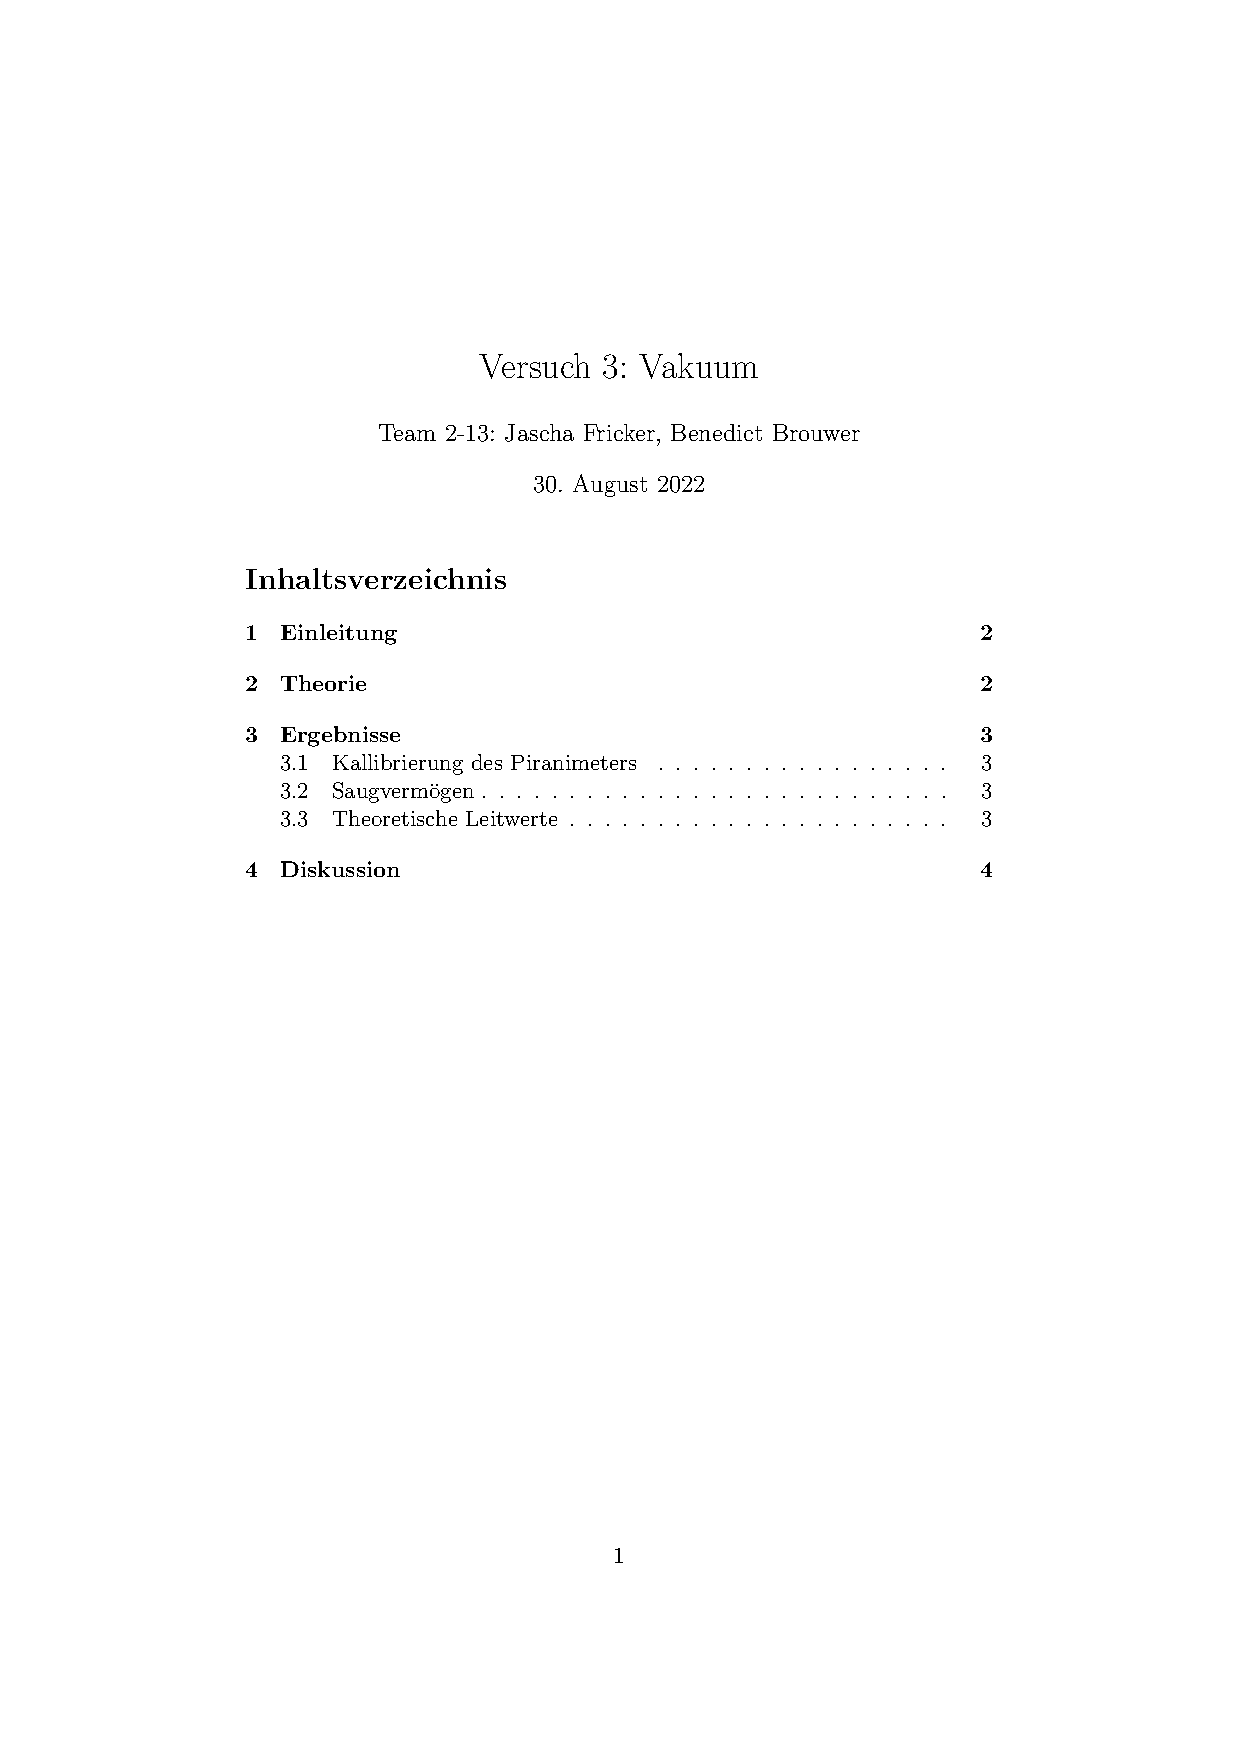
\includegraphics[width=0.8\textwidth]{VAK/VAKaus.pdf}
        \caption{Kallibrierung des Piranimeters}
        \label{fig:piranim}
    \end{figure}

    \subsection{Saugvermögen}

    \subsection{Theoretische Leitwerte}
    In der Tabelle \ref{tab:./VAK/tabelle} werden die theoretisch berechneten Leitwerte und effektive Saugleistungen der verschiedenen Konstellationen aus Schlauch und Kapillare dargestellt. Dabei wurde eine nominale Saugleistung von $S = 3,7 \si(\meter\per\hour)$ angenommen.
    \input{tabelle.txt}


    \section{Diskussion}

    \bibliographystyle{plain}
    \bibliography{literature}

\end{document}